\documentclass[../main-v2-manifolds.tex]{subfiles}


\begin{document}
%%%%%%%%%
%%%%%%%%%
%%%%%%%%%
\makeatletter
\newcommand*{\addFileDependency}[1]{% argument=file name and extension
\typeout{(#1)}% latexmk will find this if $recorder=0
% however, in that case, it will ignore #1 if it is a .aux or 
% .pdf file etc and it exists! If it doesn't exist, it will appear 
% in the list of dependents regardless)
%
% Write the following if you want it to appear in \listfiles 
% --- although not really necessary and latexmk doesn't use this
%
\@addtofilelist{#1}
%
% latexmk will find this message if #1 doesn't exist (yet)
\IfFileExists{#1}{}{\typeout{No file #1.}}
}\makeatother

\newcommand*{\myexternaldocument}[1]{%
\externaldocument{#1}%
\addFileDependency{#1.tex}%
\addFileDependency{#1.aux}%
}
%------------End of helper code--------------
%%%%%%%%
% PUT ALL EXTERNAL DOCUMENTS YOU WANT TO REFERENCE IN THIS SECTION
\myexternaldocument{./Preliminaries-Compiled} % Reference the Preliminiaries Page
%%%%%%%%%
%%%%%%%%%
%%%%%%%%%
%%%%%%%%%
\fchapter{4: Symplectic Geometry}
% Let $n\geq 1$. We will be working in $\real^{2n}$. Let us define
% \begin{itemize}
%     \item $X = C^\infty(S^1\,\realtn)$, where $S^1 = \{z\in\complex, \abs{z}=1\}$.
%     \item Recall the Sobolev space $M = H_{1/2}$ is equipped with the inner product and norm defined in \cref{eq:hofer 1/2 inner product,eq:hofer 1/2 norm}.
% \end{itemize}
% \[
%     s
% \]
% % %%%%
% Loops are always closed, and we assume all loops are $1$-periodic. We will not distinguish between $S^1$ and $\real/\mathbb{Q}$. The measure we will use on $S^1$ is the Lebesgue measure.\\
% %%%
% \topheader{Almost complex structure}
% \begin{definition}[Almost complex structure]
%     A smooth manifold $M$ of dimension $2n$ has an \emph{almost complex structure} whenever it admits a smooth 'transformation' on the tangent spaces of each $x\in M$, 
%     \[
%     J_x: T_xM \to T_xM\quad J_xJ_x = -\id{T_x{M}}
%     \]
% \end{definition}
% \begin{remark}
%     This transformation should be interpreted in the 'tensor' sense. If $n = 1$, then $J$ is a section of the $\Tau^2 TM$ bundle, so that $J_x\in L(T_xM, T_xM;\real)$ is a $2$-covariant tensor --- which can be identified as a bilinear form on each tangent space.
% \end{remark}

%%

%%
%% Custom commands for this section????
\providecommand{\symatrix}{\begin{bmatrix}
    0 & 1 \\ -1 & 0
\end{bmatrix}}
\newcommand{\bigdot}[1]{\overset{\bullet}{#1}}
\providecommand{\realtn}{{\real^{2n}}}
%%
\topheader{Primer on Differential Forms}
\begin{remark}[Finite-dimensional Manifolds]
    We assume all manifolds modelled over $\realn$ ($n\geq 1$) are of class $C^\infty$, and are equipped with Hausdorff, second-countable topologies.
\end{remark}
Let $M$ be a manifold modelled on $\realn$.
\begin{multicols}{2}
\begin{itemize}
    \item $\vField(M)$ = ($C^\infty(M)$) module of vector fields on $M$,
    \item $\cvField(M)$ = module of covector fields on $M$,
    \item $\Tau^{(j,k)}(M)$ = module of $j$-contravariant, $k$-covariant tensor fields on $M$.
    \item $\Tau^{k}(M)$ = $\Tau^{(0,k)}(M)$.
    \item $\Omega^k(M)$ = module of $k$-forms on $M$.
\end{itemize}
\end{multicols}

\begin{note}[Covariant and Contravariant Tensors]
    We recall that if $V$ is a $\real$-vector space, a $j$-contravariant, $k$-covariant tensor on $V$ --- denoted by $F$ --- is a $(j+k)$ linear mapping that takes $j$-covectors, and $k$-vectors to a real number. In symbols,
    \[
        F: (V^*)^j \times V^k\to\real\quad\text{is multilinear.}
    \]
    We denote the space of $(j,k)$ tensors on $V$ by $\Tau^{(j,k)}(V)$. The space of $(0,0)$ tensors on $V$ is identified with $\real$ --- as it depends on $0$ arguments. \\
    
    If $V$ is finite dimensional, then $V=\Tau^{(1,0)}(V)$, and $V^* = \Tau^{(0,1)}(V)$.
    Similarly, $\vField(M) = \Tau^{(1,0)}(M)$,  $\cvField(M) = \Tau^{(0,1)}(M)$ and $C^\infty(M) = \Tau^{(0,0)}(M)$.
\end{note}
If $N$ is another manifold and $u: M\to N$ a morphism, 
\begin{itemize}
    \item for every $f\in C^\infty(N)$, the \emph{pullback} through $u$ is the precomposition $u^*f = f\circ u\in C^\infty(M)$, and
    \item for every $A\in\cvField(N)$, the \emph{tensor field pullback} through $u$ is the precomposition.  It is defined by
    \[
        (u^*A)(p)(v) = A[u(p)][du(p)(v)],\quad\text{where the square brackets are for readability.}
    \]
    For a general $A\in \Tau^{k}N$, we have
    \[
        (u^*A)(p)(v_{\underline{k}}) = A[u(p)][du(p)(v_{\underline{k}})],\quad\text{for an arbitrary }p\in M,\: v_{\underline{}k}\in T_pM.
    \]
    \item If $u$ is a diffeomorphism, we define the \emph{vector field pullback} of a vector field $Y\in\vField(N)$ by
    \[
        (u^*Y)(p) = du^{-1}\qty(Y_{u(p)}) = (du^{-1}\circ Y\circ u)(p)
    \]
\end{itemize}
We recall a few facts from differential geometry.
\begin{itemize}
    \item If $f\in C^\infty(M)$, the \emph{exterior derivative} of $f$ is the covector field $df$ with coordinate representation
    \[
        df(p) = \sum_{i=\underline{n}}\pdv{f}{x^i}dx^i.
    \]
    \item If $A\in \Omega^k(M)$, the \emph{exterior derivative} of $A$ is a $k+1$ form that is defined by its local coordinate representation. 
    \item The exterior derivative $d$ commutes with the tensor field pullback. That is, for every $A\in \Omega^k(N)$, $u^*(dA) = du^*A$.
\end{itemize}
\begin{definition}[Exterior Derivative in Local Coordinates]
    Let $M$ be a manifold modelled on $\realn$, and $A\in \Omega^k(M)$. If $(x^i)$ are the local coordinates in some open subset $U\osub M$, $A$ can be written as the tensor product of dual basis vectors $(dx^i)$.
    \begin{equation}
        A = \isum_{J}A_J dx^J
        \label{eq:k form isum local representation}
    \end{equation}
    where $\isum$ refers to an increasing sum taken over $k$-indices. We define the \emph{exterior derivative of $A$} by the $k+1$ form in local coordinates
    \begin{equation}
        dA = d\qty(\isum_J A_J dx^J) = \isum_J dA_J \wedge dx^J.
        \label{eq:exterior derivative of isum local representation 1}
    \end{equation}
    Unboxing the differential of $A_J$ and the wedge product, \cref{eq:exterior derivative of isum local representation 1} becomes:
    \begin{equation}
        dA = \isum_J \sum_{i=\underline{n}}\pdv{A_J}{x^i}dx^i\wedge dx^J = \isum_J\sum_{i=\underline{n}} \pdv{A_J}{x^i}dx^{(i,J)}.
        \label{eq:exterior derivative of isum local representation 2}
    \end{equation}
\end{definition}
\begin{example}[Exterior Derivative in Coordinates]\label{exmp:exterior derivative}
    Let $M = \real^3\setminus \{0\}$, we will use the standard coordinates $(x,y,z)$ on $M$. 
    \begin{enumerate}
        \item $f(x,y,z) = (x^2 + y^2)^{1/2}$ = scalar valued function.
        \item $A(x,y,z) = (y-x)dz - zdy$ = covector field.
        \item $B(x,y,z) = f(x,y,z)dx\wedge dy$ = $2$-form.
    \end{enumerate}
    Exterior Derivative of $f$:
    \[
        df(x,y,z) = \pdv{f}{x}dx + \pdv{f}{y}dy + \pdv{f}{z}dz = \frac{xdx + ydy}{f(x,y,z)}
    \]
    Exterior Derivative of $A$:
    \begin{align*}
        dA(x,y,z) &= d(y-x)\wedge dz + d(-z)\wedge dy \\[1ex]
        &= dy\wedge dz - dx\wedge dy - dz\wedge dy = 2dy\wedge dz -dx\wedge dy
    \end{align*}
    Exterior Derivative of $B$:
    \[
        dB(x,y,z)= df(x,y,z)\wedge (dx\wedge dy) = \frac{xdx + ydy}{f(x,y,z)}\wedge (dx\wedge dy)=0
    \]
\end{example}
\begin{remark}[Exterior Derivative on Banach Manifolds]
    If $X$ is a Banach space, which is also a Banach manifold of class $C^k$ for $k\geq 1$, the exterior derivative of $C^k$ function $f$ is a $C^{k-1}$ covector field whose evaluation at $p\in X$ coincides with the Frechet Derivative $Df(p)$. Recall that $Df(p)$ is the unique linear map that satisfies
    \[
        f(p + v) = f(p) + Df(p)(v) + o(\abs{v}).
    \]
\end{remark}
\begin{remark}[Closed, and exact differential forms]
    Let $A\in \Omega^k(M)$ be a $k$-form on manifold $M$. 
    \begin{itemize}
        \item It is \emph{closed} whenever $dA = 0$, and
        \item is \emph{exact} whenever $A = dB$ where $B \in \Omega^{k-1}(M)$.
    \end{itemize}
\end{remark}
\begin{remark}[Poincare's Lemma]
    A subset $S\subseteq\realn$ is said to be \emph{star-shaped} if there exists some $a\in S$ where $\{a + (b-a)[0,1]\}\subseteq S$ for every $b\in S$. That is, the straight line segment between $a$ and every point $S$ is contained in $S$.\\

    Poincare's Lemma states that, if $U$ is an open, star-shaped subset of $\realn$, then every closed form is exact.
\end{remark}
\begin{remark}[Line integral]
    Let $\gamma: [0,L]\to M$ where $M$ is a smooth manifold. For any smooth $1$-form $\lambda$ on $M$, the integral of $\gamma$ over $\lambda$ is the integral
    \[
        \int_\gamma \lambda =  \int_{[0,L]} \gamma^*\lambda = \int_{0}^{L}\lambda(\gamma(t))(\mathring{\gamma}(t))dt.
    \]
\end{remark}
\begin{example}[Line integral in coordinates]
    Let $\gamma(t) = (\cos(2\pi t), \sin(2\pi t), 0)$ for $t\in[0,1]$, and the covector field 
    \[A(x,y,z) = \frac{xdy - ydx}{x^2 + y^2}\quad\forall (x,y)\neq 0.\]
    Suppressing the trigonometric arguments, the line integral of $A$ over $\gamma$ is given by
    \[\int_{\gamma}A = \int_{0}^{1} A[\gamma(t)][\dot{\gamma}(t)]dt = \int_0^1 \frac{\cos dy - \sin dx}{\cos^2 + \sin^2}(2\pi (-\sin, \cos,0))dt\]
    which gives
    \[\int_{\gamma} A = 2\pi\int_0^1\cos\cos - \sin(-\sin) dt = 2\pi.\]
\end{example}
%
%% Footnote: a differential form is said to be closed whenever its exterior derivative is zero.
%% Footnote: a differential form is said to be exact whenever it is the exterior derivative of another differential form.
%% Poincare's Lemma: if M is a star-shaped domain, then a differential 1-form is closed if and only if it is exact.
%% Fact: Exact forms are always closed, but closed forms are not always exact - depends on deRham cohomology.
\topheader{Standard Symplectic Form}
We begin the case in $\real^2$. The \emph{standard symplectic form} on $\real^2$ is the bilinear form represented by the matrix (with repect to the standard basis) in \cref{eq:std symplectic form r2}.
\begin{equation}
    J = \mqty[0 & 1\\ -1 & 0]
    \label{eq:std symplectic form r2}
\end{equation}
The following note summarizes several properties of $J$.
\begin{note}[Properties of the standard symplectic form on $\real^2$]\label{note:properties of std symplectic form r2}
    If $x,y\in\real^2$, \cref{eq:std symplectic form r2} defines a pairing $\omega_0\in \Omega^2(\real^2)$ between $x$ and $y$. Where $\omega_0(x,y) = \langle x, Jy\rangle_{\real^{2}}$. An easy computation in coordinates will show that
    \begin{equation}
        \omega_0(x,y) = \begin{bmatrix}x_1 & x_2
        \end{bmatrix}\begin{bmatrix}0 & 1 \\ -1 & 0\end{bmatrix}\begin{bmatrix} y_1 \\ y_2\end{bmatrix} = \det\qty(\begin{bmatrix} x_1 & y_1 \\ x_2 & y_2\end{bmatrix}) = \det(x,y)
        \label{eq:std symplectic action pw r2}
    \end{equation}
    Furthermore, 
    \begin{itemize}
        \item $J$ is non-singular and skew-symmetric, and $J^{-1} = (-1)J$.
        \item $\omega$ is non-singular and skew-symmetric, it is a non-degenerate $2$-form on $\real^{2n}$ by \cref{lem:characterisation of bilinear forms}.
        \item Left multiplication by a vector $v = (v^1, v^2)$ reads 
        and $\omega_0(v,\cdot) = v^1\varepsilon^{2} + (-1)v^2\varepsilon^1$.
        \item Right multiplication by $v$: by skew-symmetry of $J$ reads: $\omega_0(\cdot, v) = (-1)v^1\varepsilon^2 + v^2\varepsilon^1$.
    \end{itemize}    
\end{note}

\begin{definition}[Standard symplectic form]\label{def:std-symplectic-form}
    Let $n\geq 1$, the \emph{standard symplectic form} is the bilinear form defined by the matrix representation in \cref{eq:std symplectic form r2n 2}.
    \begin{equation}
        J =\begin{bmatrix}
            \admat[0]{I_n,-I_n}
        \end{bmatrix}
        \label{eq:std symplectic form r2n 2}
    \end{equation}
    The matrix in \cref{eq:std symplectic form r2n 2} induces a bilinear pairing, which we will denote by $\omega_0\in \Omega^2(\realtn)$. Its defining property is that it computes the sum of $n$ $2\times 2$ determinants, as shown in \cref{eq:std symplectic form r2n determinants}. 
    \begin{equation}
        \omega_0(x,y) =\langle x,y\rangle_{\omega_0} = \sum_{i=\underline{n}}\det\qty(\mqty[x^i & y^i \\ x^{n+i} & y^{n+i}])
        \label{eq:std symplectic form r2n determinants}
    \end{equation}
    We can rewrite $\omega_0$ using the language of differential forms:
    \begin{equation}
        \omega_0 = \sum_{i=\underline{n}}\varepsilon^{i}\wedge\varepsilon^{n+i}.
        \label{eq: std symplectic form r2n wedge products using covectors}
    \end{equation}
\end{definition}
The properties outlined in \cref{note:properties of std symplectic form r2} all hold for $\realtn$. Moreoever, $\omega_0$ is exact, as one can verify that if $\lambda = \sum x^i dx^{n+i}$ with the sum taken over $\underline{n}$, then $d\lambda = \omega_0$. Recall if $p,v\in\realtn$, 
\[
    \lambda(p) = \sum p^{i}dx^{n+i}\qqtext{and} \lambda(p)(v) = \sum p^{i}v^{n+i}.
\]
%
\begin{remark}[Alternate Symplectic Structure]
    Some texts use \cref{eq:std symplectic form r2n 1}, or $J = \mqty[0 & -I_n\\ I_n & 0]$. The following decomposition is called the \emph{maximal hyperbolic decomposition} of $\realtn$, see \cite{Roman2007Advanced} Chapter 13. We will return to this later when we discuss periodic solutions on ellipsoids.
    \begin{equation}
    J = \begin{bmatrix}
        \dmat{\symatrix,\ddots,\ddots,\symatrix}
    \end{bmatrix}
    \label{eq:std symplectic form r2n 1}
\end{equation}
\end{remark}
%
%
\begin{note}[Computations with the standard symplectic form]\label{note: symplectic form summation computations}
    We call the standard symplectic form given in \cref{eq:std symplectic form r2n 2} in terms of the Kronecker delta. A moment's thought will show that $J = [\delta_{(i,j-n)} - \delta_{(i,j+n)}]_{ij} = [\delta_{(n+i,j)} - \delta_{(i-n,j)}]_{ij}$. Left multiplication by a vector $v = (v^{\underline{2n}})$ yields
    \begin{align*}
        \omega_0(v,\cdot) &= \langle v, J\cdot\rangle_{\realtn} = v^i[\delta_{(i,j-n)} - \delta_{(i,j+n)}]\varepsilon^j\\[2ex]
        &=\sum_{i=\underline{2n}}v^i\varepsilon^{i+n} - v^i\varepsilon^{i-n} =\sum_{i=\underline{n}}v^i\varepsilon^{i+n} - v^{i+n}\varepsilon^{i}
    \end{align*}
    Right multiplication then give us 
    \[
        \omega_0(\cdot, v) = \langle \cdot,Jv\rangle_{\realtn} = \sum_{i=\underline{n}}(-1)v^i\varepsilon^{i+n} + v^{i+n}\varepsilon^i.
    \]
\end{note}
\topheader{Symplectic Manifolds}
We introduce a more differential geometric viewpoint, and work with arbitrary symplectic structures.
\begin{definition}[Symplectic Manifold]\label{def:symplectic manifold}
    A \emph{symplectic manifold} is a manifold $M$ modelled on $\realtn$ (for $n\geq 1$), equipped with a \textbf{closed, non-degenerate $2$-form $\omega$}. We sometimes refer the tuple $(M,\omega)$ as the \emph{symplectic structure}.
\end{definition}
\begin{definition}[Symplectomorphism]
    Let $(M,\omega)$ and $(N,\eta)$ be symplectic manifolds of dimension $2m$ and $2n$ respectively. A mapping $u: M\to N$ is a \emph{symplectomorphism} (or is symplectic as an adjective) whenever it preserves the symplectic structure under the tensor pullback. That is,
    \[
        u^*\eta =\omega,\qqtext{which means} \omega(p)(v_1,v_2) = \eta(u(p))\biggl(du(p)[v_1], \:du(p)[v_2]\biggr)\quad\forall p\in M,\: v_{\underline{2}}\in T_pM.
    \]
    An embedding that is a symplectomorphism is called a \emph{symplectic embedding}.
\end{definition}
\begin{example}[Symplectomorphism on $\realtn$]
Let $\varphi:\realtn\to\realtn$ be smooth, we say $\varphi$ is a \emph{symplectomorphism} (or $\varphi$ is symplectic as an adjective) whenever it preserves $\omega$. That is,
\[
    \left\langle D\varphi(x)(v_1), D\varphi(x)(v_2)\right\rangle_{\omega_0} = \omega_0(v_1, v_2)\quad\forall x,v_1,v_2\in\realtn,
\]
where $D\varphi(x)$ refers to the Jacobian matrix of $\varphi$ evaluated at $x\in\realtn$. If $\varphi$ is a $C^\infty$ diffeomorphism and $\varphi$ and its inverse are symplectomorphisms, we call $\varphi$ a \emph{symplectic diffeomorphism} or a \emph{symplectic isomorphism}.
\end{example}
%
%
%
% \begin{note}[Alternate interpretation using tensor pullbacks]
%     Equivalently, we say $\varphi$ is a symplectomorphism whenever $\omega_0$ is invariant under its tensor pullback. This means, 
%     \begin{equation}
%         \varphi^*(\omega_0) =\omega_0
%         \label{eq:symplectomorphism tensor pullback}
%     \end{equation}
%     This is the same as
%     \[
%         (D\varphi(x))^{T}J D\varphi(x) = J\quad\text{in the sense of matrix multiplication.}
%     \]
%     An immediate consequence of the previous formula is that a symplectomorphism $\varphi$ must be volume-preserving, meaning $\det D\varphi(x) = 1$ at every point.
% \end{note}
\begin{remark}
    Symplectomorphisms are volume preserving. If $\varphi:M\to N$ is a symplectomorphism, then the determinant of the Jacobian matrix (with respect to any pair of charts) is $1$.
\end{remark}
%
\begin{lemma}[Symplectomorphisms preserve the symplectic action]
    If $\varphi$ is a symplectomorphism on $\realtn$, then $A(\varphi\circ\gamma) = A(\gamma)$ for every $\gamma\in \Omega$.
\end{lemma}
\begin{proof}
    Because the exterior derivative commutes with the tensor pullback, we have
    \[
        d(\lambda - \varphi^*\lambda) = d\lambda - \varphi^*(d\lambda)= 0
    \]
    whence $\lambda - \varphi^*\lambda$ is a closed differential form. Using \cref{eq:loop space S1 r2n symplectic action lambda}, we see that
    \[
        A(\varphi\circ\gamma) - A(\gamma) = \int_{\gamma}\varphi^*\lambda - \int_{\gamma}\lambda = \int_{\gamma}(\varphi^*\lambda - \lambda)
    \]
    It follows from Poincare's Lemma that the right hand vanishes, since it is the closed curve over an exact form.
\end{proof}
\topheader{Hamiltonian Vector Fields}
We begin with some well known sign conventions for area.
\begin{quote}
    Fix any two vectors $v_1, v_2\in \realn$, we say that positive area opens anti-clockwise from $v_1$. (Draw a picture).
\end{quote}
Because of this, we refer to $\det(v_1, v_2)$ as the \emph{area spanned from $v_1$ to $v_2$} if $v_1,v_2\in\real^2$, and we call $\omega_0(v_1,v_2)$ the \emph{symplectic area from $v_1$ to $v_2$}. Moreoever, if $S$ is a compact region in $\realn$ whose (topological or manifold) boundary $\partial S$ can be traversed by a continuous curve $\gamma:[0,1]\to\realn$. 
\begin{quote}
We say $\gamma$ is positively oriented (with respect to the \emph{Stokes' orientation}), whenever the region $S$ lies to the left of $\gamma$ at every point.
\end{quote}
\begin{figure}[h!]
    \centering
    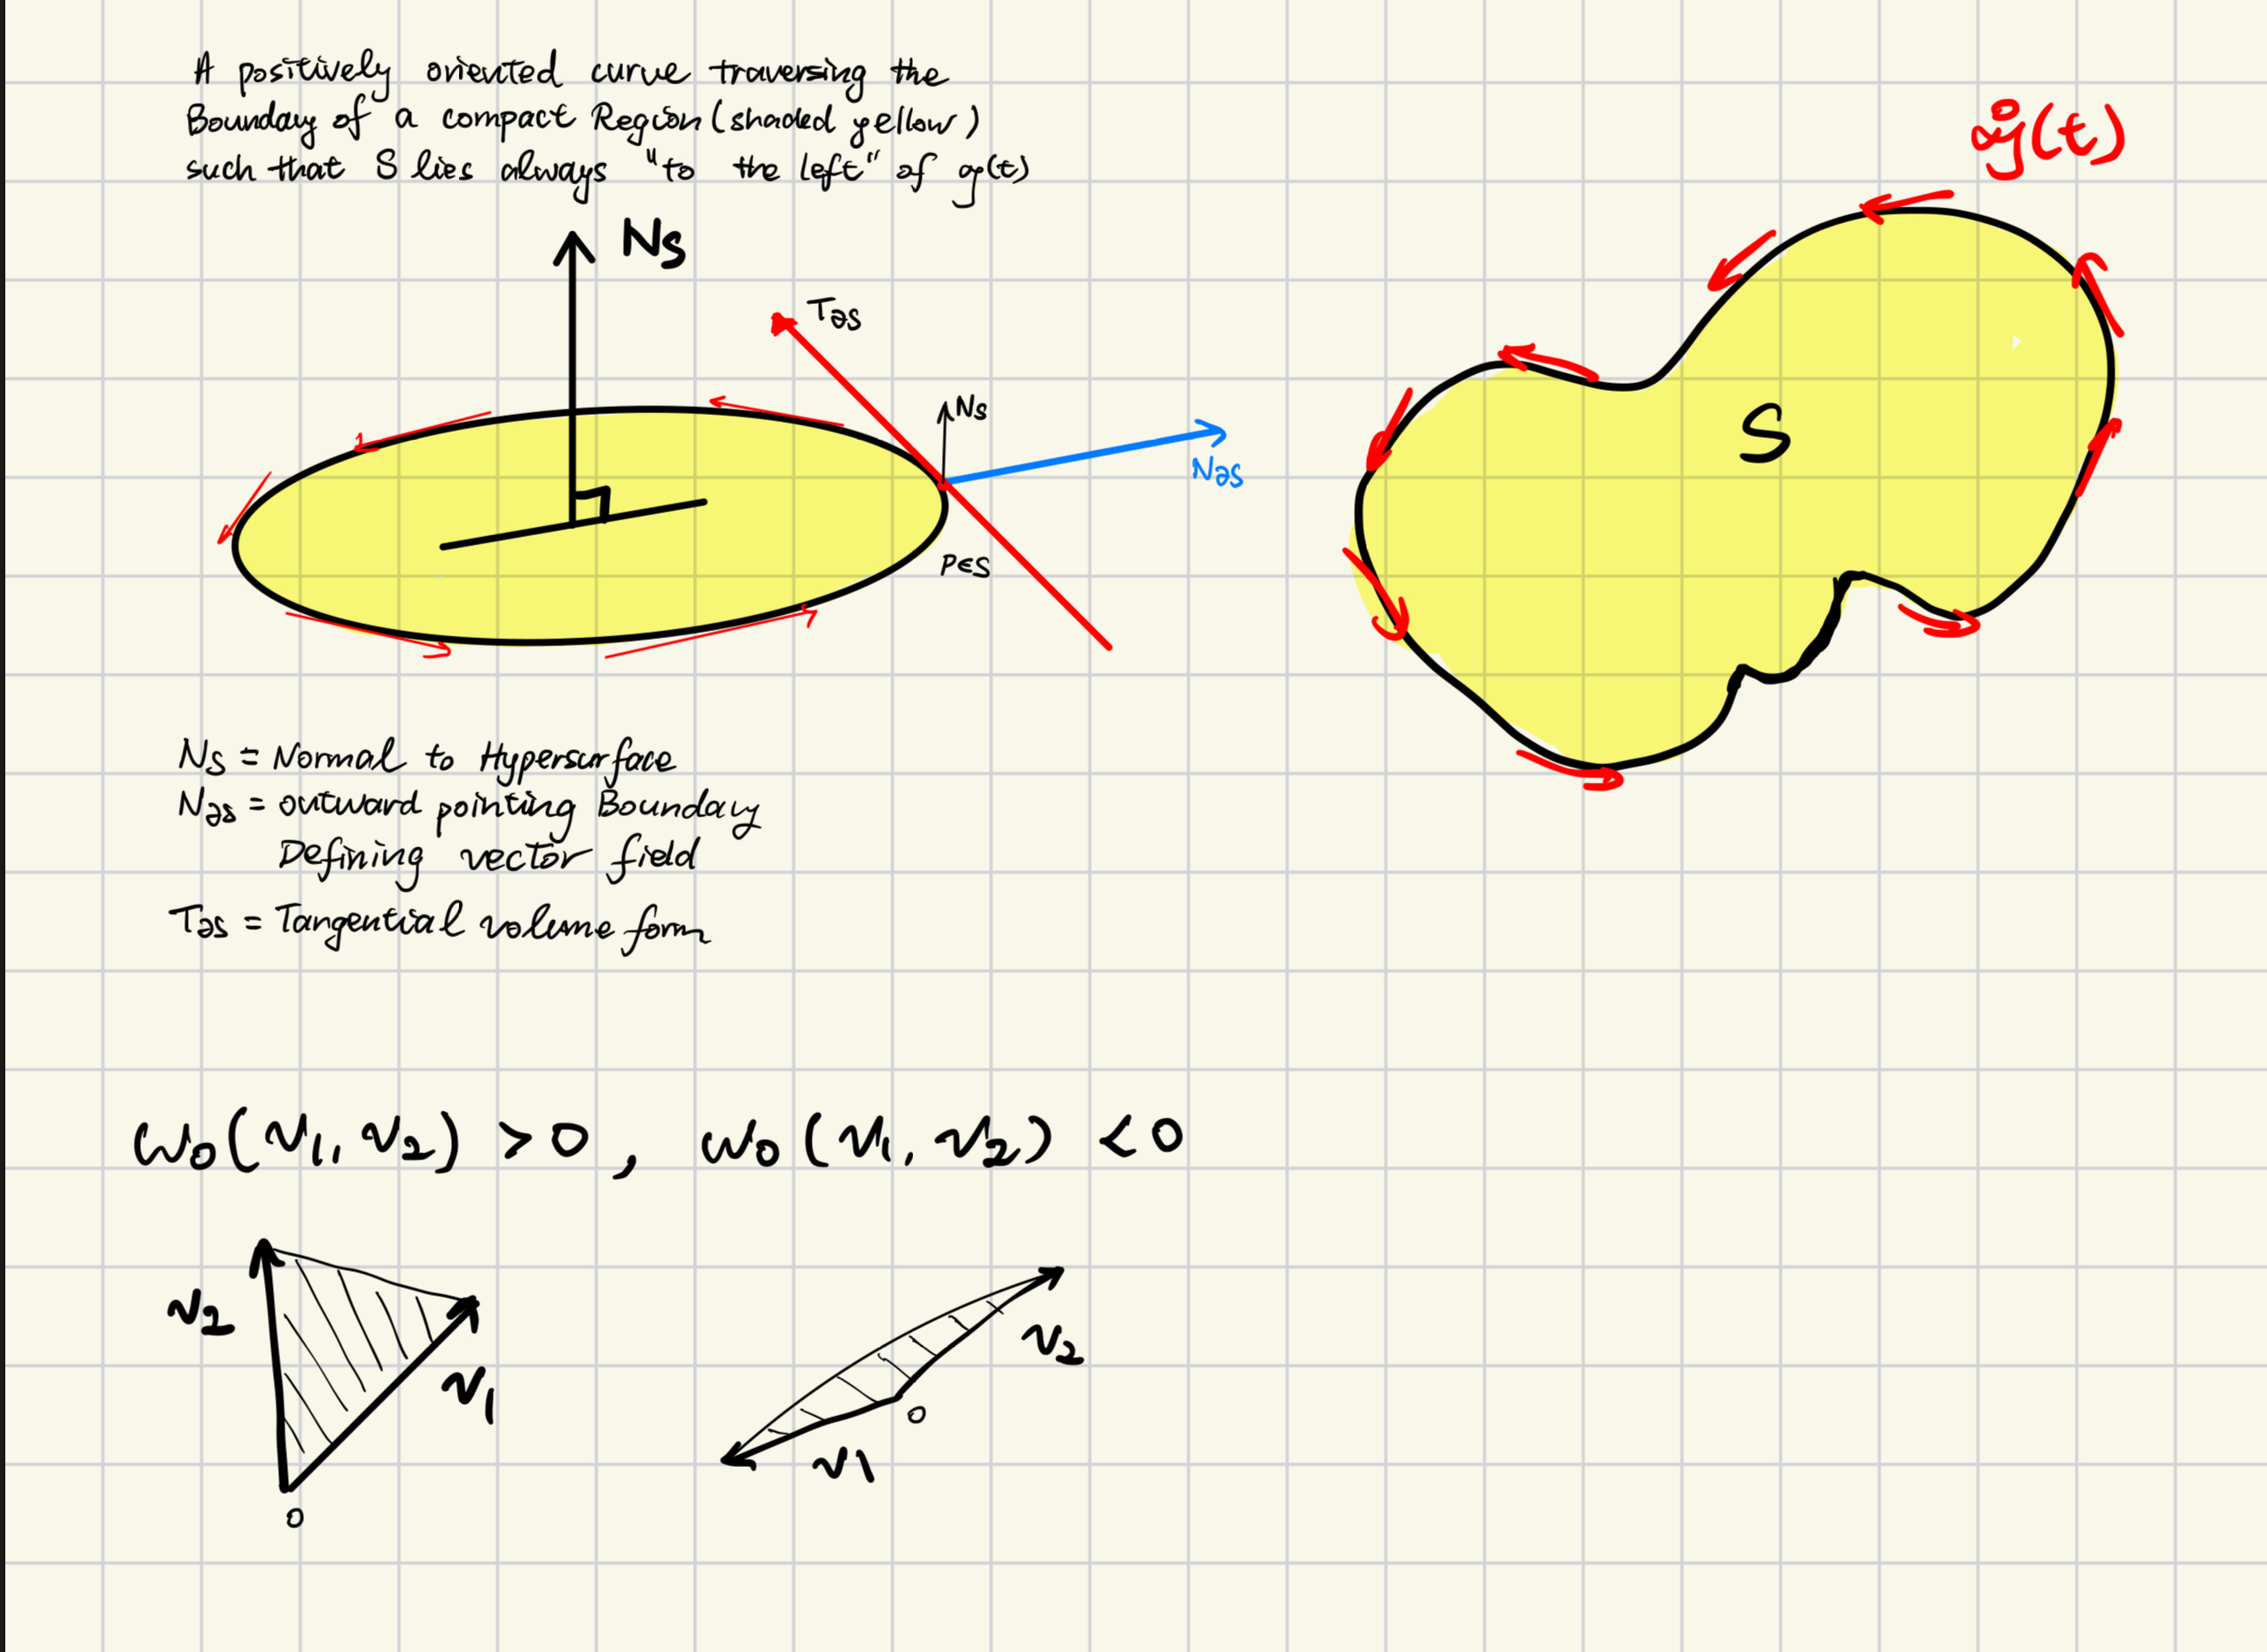
\includegraphics[width=0.5\linewidth]{images/positive-area-opens-to-left-sketch.png}
    \caption{Illustrations of area sign conventions}
    \label{fig:area sign conventions}
\end{figure}
\begin{remark}[Positive Gradient Flow]\label{rmk:gradient flow}
Let $H\in C^\infty(\realtn)$, the \emph{positive gradient flow} of $H$ is the vector field $\nabla H$ such that at every point $p\in \realtn$, and $v_p\in T_p \realtn$:
\begin{quote}
    The \textbf{angle between $\nabla{H}(p)$ and $v_p$ is equal to $DH(p)(v_p)$}, where
    \begin{equation}
    H(p+v_p) = H(p) + DH(p)(v_p) + o(\abs{v_p})\quad\text{for sufficiently small }v.
    \label{eq:Frechet Derivative as best possible linear approximation}
\end{equation}
\end{quote}
By the 'angle' we refer to the Euclidean inner product which takes on values in $\real$ instead of in $[-\pi, +\pi]$. Moreover, the \emph{Euclidean gradient} of $H$ in coordinates is given by
\[\nabla H = (\partial_{\underline{2n}}H)\in\vField(\realtn).\]
\end{remark}
\begin{definition}[Hamiltonian Flow]
    The \emph{Hamiltonian flow} of $H$ is the vector field $X_H$ such that at every point $p\in \realtn$, and $v_p\in T_p\realtn$:
    \begin{quote}
        The \textbf{symplectic area from $X_H(p)$ to $v_p$ is equal to $DH(p)(v_p)$.}
    \end{quote}
    More precisely, the Hamiltonian flow of $H$ is defined by the sharpening the covector field of $H$:  $X_H = \omega_0^{\wedge}(dH)$, such that
    \begin{equation}
        \omega_0(X_H(p), v_p) = dH(p)(v_p)\quad\text{for all }p\in \realtn,\: v_p\in T_p\realtn.
        \label{eq:hamiltonian flow definition symplectic pairing}
    \end{equation}
\end{definition}
In Euclidean space, $X_H$ has a simple structure, and is related to the $\nabla H$ by a factor of $J$. 
\begin{lemma}[Hamiltonian Flows in Euclidean Space]\label{lem:hvf in euclidean space formula}
    The Hamiltonian flow of $H\in C^\infty(\realtn,\real)$, $X_H$ has matrix representation which satisfies
    \begin{equation}
        X_H = J\nabla H.
        \label{eq: hvf in euclidean space formula}
    \end{equation}
\end{lemma}
\begin{proof}
    Let $p$ and $v_p$ be arbitrary, it follows from the definition of $X_H$ that
    \[
        \langle X_H(p), v_p\rangle_{\omega_0} = \langle X_H(p), Jv_p\rangle_{\realtn} = dH(p)(v_p) = \langle\nabla H(p), v_p\rangle_{\realtn}.
    \]
    Notice that $J$ is skew-symmetric, so we can move $J$ over to the other side of the bracket at the cost of a minus sign, hence:
    \[
        \langle (-1)J X_H(p), v_p\rangle_{\realtn} = \langle \nabla H(p),v_p\rangle_{\realtn}.
    \]
    The proof is complete upon seeing that $(-1)J=J^{-1}$.
\end{proof}
\begin{remark}
    If $X_H$ is a Hamiltonian flow, we sometimes refer to its integral curves as \emph{solutions}. If a solution is periodic, it is called an \emph{orbit} of $X_H$.
\end{remark}
\topheader{Statement of the Weinstein's Conjecture}
\begin{definition}[Closed submanifold]\label{def:closed-submanifolds}
    Let $M$ be a manifold modelled on $\realn$. A submanifold $S\subseteq M$ is said to be \emph{closed} whenever it is a compact subset of $M$, and the $S$ is a manifold without boundary.
\end{definition}
\begin{remark}[Stokes' Theorem]
    Let $M$ be a manifold with boundary modelled on $\realtn$, for any compactly supported $(n-1)$ form $\omega$:
    \begin{quote}
        The integral of $d\omega$ over $M$ is equal to the integral of $\omega$ over $\partial M$. In symbols,
        \[\int_{M}d\omega = \int_{\partial M}\omega.\]
    \end{quote}
    If $S$ is a closed submanifold of $M$, and $\omega$ a $(n-1)$-form, an immediate corollary is that
    \[\int_S d\omega = \int_{\partial S}\omega = 0.\]
\end{remark}
\begin{definition}[Regular hypersurface]\label{def:regular hypersurface}
    A \emph{regular hypersurface} on a smooth manifold $M$ is a subset $S = f^{-1}(c)$ where $f\in C^\infty(M,\real)$, and $df(p)\neq 0$ for every $p\in S$. We call $f$ the \emph{defining function} of $S$ which admits a natural manifold structure that makes $S$ a submanifold of $M$. 
\end{definition}
\begin{definition}[Energy surface]\label{def:energy surface}
    An \emph{energy surface} is a compact, regular hypersurface of a symplectic manifold $(M,\omega)$.
\end{definition}
We conclude this section by stating Weinstein's conjecture on $\realtn$.
\begin{quote}
    Does every energy surface on $(\realtn,\omega_0)$ admit a non-degnerate, closed orbit?
\end{quote}
A more abstract reformulation of the conjecture is given below.
\begin{quote}
    Given an energy surface $S$, does its line bundle $\mathcal{L}(S)$ admit a closed characteristic?
\end{quote}
Where $\mathcal{L}(S) = \bigset{(x,v)\in TS,\:  v\in \rad{\omega_0(p)}}$ and a \emph{closed characteristic} of $S$ refers to a $1$-dimensional submanifold that is diffeomorphic to the $1$-sphere.
\begin{wts}[WC Reduction 1 --- Independence of Hamiltonian]\label{thm:wc reduction 1 hamiltonian}
    Let $S$ be a compact, regular hypersurface on a symplectic manifold $(M,\omega_0)$. If $F, G\in C^\infty(M)$ are defining functions of $S$ such that
    \[S = F^{-1}(c) = G^{-1}(c'),\]
    where 
    \[dF(x)\neq 0\qqtext{and}dG(x)\neq 0\quad\forall p\in S.\]
    Then, there exists a $\rho\in C_c^\infty(M,\real)$ that satisfy the following
    \begin{itemize}
        \item For every $x\in S$, $\rho(x)\neq 0$ and $dF(x) = \rho(x) dG(x)$.
        \item For any $x\in S$, let $\varphi_x(s) = \varphi(s,x)$ and $\theta_x(t) = \theta(t,x)$ denote the integral curves starting at $x$ of $X_F$ and $X_G$. The smooth function $\alpha$ constructed by solving the IVP in \cref{eq:wc reduction1: alpha reparam} relates the two flows by its reparametrization.
        \begin{equation}
            \dv{\alpha}{s} = \rho(\varphi_x(s))\quad\alpha(0)=0
            \label{eq:wc reduction1: alpha reparam}
        \end{equation}
        By reparametrization we mean that $\varphi_x(s) = \theta_x(\alpha(s))$ for all $s$ whenever either side is defined.
        \item The periodic orbits of $X_{F}$ and $X_G$ on $S$ correspond bijectively.
        \item For any $x\in S$, $\varphi_x$ is a non-degenerate periodic orbit if and only if $\theta_x\circ\alpha$ is.
    \end{itemize}
\end{wts}
\begin{proof}
    Both $F$ and $G$ are global defining functions of the submanifold $S$, if $p\in S$ is arbitrary, the exterior tangent space coincides precisely with $\Ker dF(p) = \Ker dG(p) = T^{\mathrm{ext}}_{p}(S)$. (Lee 5.38, 5.40). Since $T^{\mathrm{ext}}_{p}S$ has dimension $1$, there exists a suitably chosen coordinate chart $(U, \zeta)$ about $p$ such that $dz\in\cvField(\real)$ spans the coordinate representation of $\cvField(T_p(S))$, and there exists smooth functions $u_F$ and $u_G$ where
    \[
        \zeta(dF(q)) = u_F(q)dz\qqtext{and}\zeta(dG(q)) = u_G(q)dz\quad\text{locally.}
    \]
    This uniquely defines $\rho$ on a neighbourhood of $p$ (by definition of the abstract tangent space), we can assume $\rho$ is compactly supported by appealing to Urysohn's Lemma for smooth manifolds.\\

    The symplectic form is $C^\infty(M)$-linear, hence $X_F = \rho X_G$ on a precompact neighbourhood of $S$. Given a point $x\in S$, we see that
    \[
        \varphi_x(s) = X_F(\varphi_x(s)) = \rho(\varphi_x(s)) X_G(\varphi_x(s)).
    \]
    Using \cref{eq:wc reduction1: alpha reparam}, we can define a smooth function $\alpha$ (because $\rho$ is smooth). Using the chain rule, and suppressing $\varphi_{x}(s)$:
    \[
        \dv{s} \theta_{x}(\alpha(s))\eval_s = \rho X_G = X_F
    \]
    So that $\theta_{x}\circ \alpha$ is an integral curve of $X_F$ starting at $x$, and must be equal to $\varphi_{x}$ by uniqueness. Next, 
    \begin{itemize}
        \item if $\theta_{x}(\alpha(s))$ is a periodic orbit of $X_G$, it follows that $\varphi_x(s)$ is a periodic orbit of $X_F$; and
        \item because $\rho$ is either strictly positive or negative, $\varphi_{x}(s)$ is a critical point of $X_F$ iff $\theta_{x}(\alpha(s))$ is a critical point of $X_G$.
    \end{itemize}
    At last, if $X_F = \rho X_G$ about $S$, then $X_G = \rho^{-1} X_F$. Let $\beta(x,t) = \int_0^t \rho(x,u)^{-1}du$, and we obtain
    \[
        \dv{t}\varphi_{x}(\beta(t))\eval_t = \rho^{-1}X_F = X_G,
    \]
    and rehearsing the same argument we had for $\alpha$ completes the proof.
\end{proof}

%
%
%
% \topheader{Symplectic Manifold}
% Let $n\geq 1$ be an integer, a \emph{symplectic manifold} of class $C^\infty$ is a real manifold of dimension $2n$ that is equipped with a $2$-form $\omega\in \Omega^2(M)$ such that
% \begin{itemize}
%     \item $\omega$ is non-degenerate, that is: at every $x\in M$ for every tangent vector $v_1\in T_xM$ there exists another tangent vector $v_2\in T_xM$ such that $\omega(v_1,v_2)$. Alternatively, the flat map is non-singular --- meaning
%     \[
%         \breve{\omega}(v_1) = \omega(v_1,\cdot) \neq 0\in T^*_xM\quad\forall v_1\in T_xM
%     \]
%     \item $\omega$ is closed, meaning $d\omega=0$ where $d$ refers to the exterior derivative of $\omega$.
% \end{itemize}
% We call a $2$-form that satisfies the two properties above a \emph{symplectic form} on $M$. 
% \begin{remark}
%     All finite-dimensional manifolds hereinafter will be assumed $C^\infty$.
% \end{remark}
%
%
%
\topheader{Symplectic Action}
We return to a more abstract-analytic perspective. Let $(X,\mcal,\mu)$ be a measure space, suppose $\gamma, \eta: X\to \realtn$ is an $L^2$ function, in the sense that it is $L^2$ in each coordinate. Holder's inequality tells us that
\[
    \langle \gamma,\eta\rangle_{\omega_0} = 2^{-1}\int_{X}\langle \gamma(x),\eta (x)\rangle_{\omega_0} d\mu(x)\quad\text{converges absolutely.}
\]
With this, we can extend the symplectic form $\omega_0$ to $L^2$ mappings into $\realtn$. The following is a natural function space to consider.
\begin{definition}[Loop Space]
    We define the space of \emph{loops} as the function space $\Omega = C^\infty(S^1, \realtn)$. It is equipped with the \emph{symplectic pairing}, which is also by $\omega_0:\Omega\times\Omega\to\real$. Given $x,y\in\Omega$, $\omega_0(x,y)$ is defined by the integral in \cref{eq:loop space S1 r2n symplectic pairing}.
    \begin{equation}
        \langle x,y\rangle_{\omega_0}= 2^{-1}\int_{S^1} \langle \mathring{x}(t), y(t) \rangle_{\omega_0} dt\quad\forall x,y\in\Omega.
        \label{eq:loop space S1 r2n symplectic pairing}
    \end{equation}
    \Cref{eq:loop space S1 r2n symplectic pairing} can be rewritten explicitly as the sum of half-determinants, which we now give
    \begin{equation}
        \langle x,y\rangle_{\omega_0} = 2^{-1}\int_{S^1} \sum_{i=\underline{n}}\det\qty(\mqty[\dot{x}_i & y_i \\ \dot{x}_{n+i} & y_{n+i}]).
        \label{eq:symplectic pairing loops r2n determinant formula}
    \end{equation}
    A simple application of Holder's inequality will show that, for every $x,y\in\Omega$, we have
    \[
        \abs{\langle x,y\rangle_{\omega_0}}\leq 2^{-1}\sum_{i=\underline{n}}\norm{y_i\dot{x}_{n+i}}_{L^2} + \norm{y_{n+i}\dot{x}_{i}}_{L^2}.
    \]    
\end{definition}
\begin{definition}[Symplectic Action]\label{def:symplectic action closed curves}
    The \emph{symplectic action} (on closed curves) is a mapping $A:\Omega\to\real$ which \textbf{computes the area swept by the curve}. 
    \begin{itemize}
        \item For an arbitrary loop $\gamma\in\Omega$, its action $A(\gamma)$ is given by \cref{eq:loop space S1 r2n symplectic action}:
        \begin{equation}
            A(\gamma) = 2^{-1}\int_{S^1}\langle\mathring{\gamma},\gamma\rangle_{\omega_0} = 2^{-1}\int_{S^1}\det\qty(\mqty[\mathring{\gamma}^{i} & \gamma^{i}\\ \mathring{\gamma}^{n+i} & \gamma^{n+i}])dt
            \label{eq:loop space S1 r2n symplectic action}
        \end{equation}
        \item or in terms of determinants, 
        \begin{equation}
            A(\gamma) = 2^{-1}\int_{S^1}\sum_{i=\underline{n}}\det\qty(\mqty[\mathring{\gamma}^i & \gamma^i \\ \mathring{\gamma}^{n+i} & \gamma^{n+i}]).
            \label{eq:loop space S1 r2n symplectic action determinant formula}
        \end{equation}
    \end{itemize}
\end{definition}
\begin{lemma}[Symplectic Action in terms of $\lambda$]
    The symplectic action, as defined in \cref{eq:loop space S1 r2n symplectic action} on $\Omega$ is also given by the line integral over $\lambda$.
    \begin{equation}
        A(\gamma) = \int_{\gamma}\lambda
        \label{eq:loop space S1 r2n symplectic action lambda}
    \end{equation}
\end{lemma}
\begin{proof}
    We expand \cref{eq:loop space S1 r2n symplectic action determinant formula} to obtain 
    \begin{equation}
        A(\gamma) = 2^{-1}\int_{S^1} \sum_{i =\underline{n}} \gamma^i\mathring{\gamma}^{n+i} - \mathring{\gamma}^{i}\gamma^{n+i} 
        \label{eq:action lambda step1}
    \end{equation}
    Notice that the first term $\int_{S^1} \sum_{i=\underline{n}} \gamma^i\mathring{\gamma}^{n+i}$ is equal to $2^{-1}\int_\gamma \lambda$. Indeed,
    \[
        \int_{\gamma}\lambda = \int_{0}^1 \lambda(\gamma(t))(\mathring{\gamma}(t)) dt = \int_{S_1} \sum_{i=\underline{n}}\gamma^i\mathring{\gamma}^{n+i}
    \]
    Using integration by parts, the integral over the each of the second terms in \cref{eq:action lambda step1} evaluates to
    \[
        2^{-1}\int_{S^1} \sum_{i=\underline{n}} \mathring{\gamma}^{i}\gamma^{n+i}=2^{-1}\sum_{i=\underline{n}}\gamma^{i}\gamma^{n+i}\eval_{\partial S^1} - 2^{-1}\int_{S^1}\sum_{i=\underline{n}}\mathring{\gamma}^{n+i}\gamma^{i}
    \]
    The boundary terms disappear since $\gamma$ is periodic, and we notice that the left hand side of \cref{eq:action lambda step1} is the sum of $2^{-1}\int_\gamma\lambda + 2^{-1}\int_{\gamma}\lambda$, and the proof is complete.
\end{proof}
%
%
%
\begin{remark}[General loops with period $L$]
    More generally, if we have two loops of period $L$ \cref{eq:loop space S1 r2n symplectic action} suggests that we can descend $\omega_0$ to an even larger space.
    \begin{equation}
        \Omega_{[0,L]} = C^\infty(\real/L\mathbb{Z}, \realtn)
        \label{eq:[0,L] r2n space}
    \end{equation}
    with $A_{[0,L]}(\gamma,\eta) = A(\gamma(Lt),\eta(Lt))$ which evaluates to
    \begin{equation}
     A_{[0,L]}(\gamma,\eta) = \frac{1}{2L}\int_{0}^{L}\langle \mathring{\gamma}(t),\eta(t)\rangle_{\omega_0}dt
     \label{eq:[0,L] r2n symplectic action}
    \end{equation}
\end{remark}

%
%
%
%
%
%
\begin{note}[$L^2$ descent of bilinear forms]
    The argument in this section about descending symplectic (resp. orthogonal) geometries onto $L^2$ functions \emph{into} the space is one of the reasons why $L^2$ functions are of such importance. To recapitulate:
    \begin{itemize}
        \item Given a bilinear form $\upsilon$ on $\real$, we can extend it to $\realtn$ for $n\geq 1$ using a 'hyperbolic decomposition' similar to \cref{eq:std symplectic form r2n 1}.
        \item This bilinear form on $\realtn$ descends into a bilinear form on the space of $L^2$ $1$-periodic loops from $S^1$ into $\realtn$,
        \item Since every loop with period $L$ admits a $1$-periodic representation, $\upsilon$ further descends to a bilinear form on $L^2([0,L], \realtn)$. Whose action is defined by the integral
        \[
            \langle \gamma,\eta\rangle_{\upsilon} = \frac{1}{2L}\int_{0}^{L}\langle\gamma(t),\eta(t)\rangle_{\upsilon}dt
        \]
    \end{itemize}
\end{note}
\begin{wts}[WC Reduction 2 --- Independence of the Symplectic Structure]\label{thm:wc reduction 2 symplectic structure }
    Suppose $(M,\omega)$ and $(N,\eta)$ are symplectic manifolds modelled on $\realtn$, and $u:M\to N$ is a symplectomorphism. 
    \begin{quote}
        To every function $F\in C^\infty(N)$, the vector field pullback of the Hamiltonian flow of $F$ is equal to the Hamiltonian flow of its pullback through $u$.     
    \end{quote}
    More precisely, if $X_F = \eta^{\wedge}(dF)$ and $u^*F = F\circ u$, we claim that
    \begin{equation}
        \omega^{\wedge}(d(u^* F)) = u^*(\eta^{\wedge}(dF))\qqtext{where} u^*(\eta^{\wedge}(dF)) = du^{-1}\circ X_F\circ u.
        \label{eq:reduction 2 eq1}
    \end{equation}
    If $\gamma$ is an integral curve of $X_{F\circ u}$, then $u\circ \gamma$ is an integral curve of $X_F$, and if $\varphi(s,x)$ and $\theta(t,y)$ denote the flows of $X_{F\circ u}$ and $X_{F}$, they relate to each other by $u$-conjugation as in \cref{eq:reduction 2 eq2}
    \begin{equation}
        u\circ\varphi^t = \theta^t\circ u.
        \label{eq:reduction 2 eq2}
    \end{equation}
\end{wts}
\begin{proof}
    Let $F$ be fixed, and write $A = dF$. Recall $d(F\circ u) = dF\circ du$. It suffices to show that
    \begin{equation}
        \omega^{\wedge}(u^* A) = u^*(\eta^{\wedge} A).
        \label{eq:reduction 2 eq3}
    \end{equation}
    We will show the left and right hand sides are equal at every tangent space. Given $p\in M$, we write
    \[X_p = \omega^{\wedge}(u^* A)(p) \qqtext{and} Y_p = u^*(\eta^{\wedge} A)(p).\]
    If $Z_p\in T_pM$ is arbitrary, we compute $\omega(p)(X_p, Z_p)$ and $\omega(p)(Y_p, Z_p)$ and the proof is complete upon showing equality. Now,
    \[\omega(p)\biggl(X_p, Z_p\biggr) = \eta(u(p))\biggl(du(p)(X_p),\: du(p)(Z_p)\biggr)= A(u(p))\biggl(du(p)(Z_p)\biggr).\]
    Using the same technique of exchanging $\omega(p)$ with $\eta(u(p))$, we get
    \[
        \omega(p)\biggl(Y_p, Z_p\biggr) = \eta(u(p))\biggl(du(p)(Y_p),\: du(p)(Z_p)\biggr),
    \]
    since $Y_p = (du^{-1}\circ \eta^{\wedge}A \circ u)(p)$, we obtain
    \[
        \omega(p)\biggl(Y_p, Z_p\biggr) = \eta(u(p))\biggl(\eta^{\wedge}A(u(p)),\: du(p)(Z_p)\biggr),
    \]
    which implies $X_p = Y_p$. This proves the first claim, and 
    \[
        du\circ X_{F\circ u} = X_F\circ du.
    \]
    Next, if $\gamma$ is an integral curve of $X_{F\circ u}$, then $\mathring{\gamma}(t) = X_{F\circ u}(\gamma(t))$ implies
    \begin{align*}
        \dv{t}u\circ \gamma(t)\eval_t &= du(\gamma(t))(X_{F\circ u}) = du\circ X_{F\circ u}\eval_{\gamma(t)} \\
        &= (X_F\circ u)\eval_{\gamma(t)} = X_F\eval_{u\circ \gamma(t)}
    \end{align*}
    and $u\circ \gamma$ is an integral curve of $X_F$. \Cref{eq:reduction 2 eq3} is proven upon realizing that $X_F$ and $X_{F\circ u}$ are $u$-related (Theorem 9.13 of \cite{Lee2013Introduction}).
\end{proof}
\begin{corollary}
    Let $M,N$ and $u$ be as in \Cref{thm:wc reduction 2 symplectic structure }, the orbits of $X_F$ correspond bijectively to the orbits of $X_{F\circ u}$ through conjugation; and the same for the non-degenerate orbits.
\end{corollary}


\ifSubfilesClassLoaded{%
  \bibliography{Functional-Analysis/manifolds-references.bib}%
}{}
\end{document}